% !Mode::"TeX:UTF-8"

% -------------------- Information --------------------

\newcommand{\TITLE}{\LaTeX 文章模板}
\newcommand{\AUTHOR}{Jason}
\newcommand{\SUBJECT}{文章模板}
\newcommand{\KEYWORDS}{}

% -------------------- Packages --------------------

\documentclass[a4paper, 12pt]{ctexart}
\usepackage{amsmath}
\usepackage{amssymb}
% \usepackage{amsthm} % 定理格式 由ntheorem代替.
\usepackage{authblk} % 作者 (见校赛论文).
\usepackage{array}
\usepackage{bigfoot} % to allow verbatim in footnote.
\usepackage{bm} % \bm for bold symbols.
\usepackage{boldline} % 长表格表格线加粗.
\usepackage{booktabs}
\usepackage{caption} % 题注.
\usepackage{commath} % abs, norm
\usepackage{enumerate}
% \usepackage{enumitem} 用enumerate包代替.
\usepackage{fancyhdr} % 脚注.
\usepackage{filecontents}
\usepackage{flafter} % 不让float出现在定义之前的地方.
\usepackage{float} % 你们这帮float给我乖乖听话 HHHHHHHHHHH.
\usepackage{fontspec} % 字体.
\usepackage{graphicx}
\usepackage{hyperref}
\usepackage{lastpage}
\usepackage{letltxmacro} % \let
\usepackage{lipsum}
\usepackage{listings} % 排版程序语言.
\usepackage{longtable} % 长表格.
% \usepackage{makecell} % 表格线加粗 \Xhline{1.2pt}. 用booktabs包代替.
\usepackage{mathtools} % \xleftrightarrow.
\usepackage{mathrsfs} % \mathscr
\usepackage{multirow} % 合并单元格.
\usepackage[square, numbers, sort&compress]{natbib} % 引用.
\usepackage[thmmarks, amsmath, thref]{ntheorem} % 定理格式.
\usepackage[section]{placeins} % 使图像不会显示在别的部分 若过于严格则换成[below].
\usepackage{stackrel} % 上下写 见校赛论文.
\usepackage{subcaption} % subcaption and subfigure
% \usepackage{SUBSubsubsection}
\usepackage{titlesec} % Section标题格式.
\usepackage{varioref} % For Cross References.
\usepackage[dvipsnames]{xcolor} % 颜色声明.
\usepackage{xfrac} %\sfrac{}{}
\usepackage[all, cmtip]{xy} % Commutive diagram.

% Require `ntheorem'

\usepackage[mathlines, edtable]{lineno} % Line numbers.
    %\begin{edtable}{tabular}[<args>] <entries> \end{edtable}

% Require `xcolor'

\usepackage[numbered, framed]{matlab-prettifier}
\usepackage{pgfplots}
\usepackage{pgfplotstable}
\usepackage{tikz}

% Incompatible with `matlab-prettifier'

\usepackage[printwatermark]{xwatermark} % Foreground Watermarks.

% -------------------- Settings --------------------

% Title

\title{\TITLE}
\author{\AUTHOR}
\date{\today}

% Package: caption

\captionsetup{
    margin    =   6pt,
    font      =   small,
    labelfont =   bf
}

% Package: ctex

\setCJKfamilyfont{fzstk}{FZShuTi} % 方正舒体
\newcommand{\fzstk}{\CJKfamily{fzstk}}

% Package: fancyhdr

\setlength{\headheight}{15pt}
\lhead{Copyright \copyright\ \AUTHOR}
\rhead{Page \thepage\ of \pageref{LastPage}}

% Package: graphicx

\graphicspath{{resources/}} % 图像文件目录

% Package: hyperref

\hypersetup{
    linktoc             =   all,
    colorlinks          =   true,
    linkcolor           =   cyan,
    anchorcolor         =   black,
    citecolor           =   green,
    filecolor           =   cyan,
    menucolor           =   red,
    runcolor            =   filecolor,
    urlcolor            =   magenta,
	pdftitle           	=   {\TITLE},
	pdfauthor          	=   {\AUTHOR},
	pdfsubject         	=   {\SUBJECT},
	pdfcreator			=	{Visual Studio Code},
	pdfproducer			=	{XeLaTeX with documentclass ctexart},
	pdfkeywords        	=   {\KEYWORDS},
    bookmarksnumbered   =   true,
    pdfstartview        =   FitH,
    pdfpagelayout       =   OneColumn
}

% Package: lineno

\renewcommand{\linenumberfont}{\normalfont\scriptsize\sffamily}

\let\oldlstinputlisting\lstinputlisting
\renewcommand{\lstinputlisting}[2][\empty]{
    \par\nolinenumbers\oldlstinputlisting[#1]{#2}\linenumbers\par
}

\let\oldlstlisting\lstlisting
\let\oldendlstlisting\endlstlisting
\renewenvironment{lstlisting}
    {\par\nolinenumbers\oldlstlisting}
    {\oldendlstlisting\endnolinenumbers\par}

\let\oldtable\table
\let\oldendtable\endtable
\renewenvironment{table}
    {\par\nolinenumbers\oldtable}
    {\oldendtable\endnolinenumbers\par}

% Package: listings

%% Title

\renewcommand\lstlistingname{代码}
\renewcommand\lstlistlistingname{代码}

%% Lstinline with color box

\LetLtxMacro{\oldlstinline}{\lstinline}
\renewcommand{\lstinline}[2][]{\colorbox{lightgray}{\oldlstinline[#1]{#2}}}
\newcommand{\matlabinline}[1]{
    \lstinline[style=MATLAB-editor, basicstyle=\mlttfamily]{#1}}

\lstset{
    breaklines=true,
    backgroundcolor=\color{lightgray},
    basicstyle=\scriptsize,
    inputpath=resources/,
    numbers=left,
    numberstyle={\color{black!33}\scriptsize\sffamily},
    xleftmargin=2em,
    xrightmargin=2em
}

% Package: ntheorem

%% Theorem
\newtheorem{theorem}{Theorem}[section]
\newtheorem{lemma}[theorem]{Lemma}
\newtheorem{corollary}[theorem]{Corollary}
%% Problem
\theoremstyle{plain}
\newtheorem{problem}{Problem}[section]
%% Proposition
\newtheorem{proposition}{Proposition}[section]
%% Conjecture
\newtheorem{conjecture}[proposition]{Conjecture}
%% Definition
\theoremstyle{plain}
\theoremheaderfont{\bfseries}
\theorembodyfont{\rmfamily}
\newtheorem{definition}{Definition}[section]
%% Note
\theoremstyle{plain}
\theoremheaderfont{\itshape}
\theorembodyfont{\itshape}
\newtheorem{note}{Note}[section]
%% Proof
\theoremstyle{nonumberplain}
\theoremheaderfont{\itshape}
\theorembodyfont{\upshape}
\theoremseparator{.}
\theoremsymbol{\ensuremath{\square}}
\newtheorem{proof}{Proof}
%% Solution
\theoremsymbol{\ensuremath{\blacksquare}}
\newtheorem{solution}{Solution}

% Package: pgfplots

\pgfplotsset{width=7cm, compat=1.16}

% Package: pgfplotstable

\pgfplotstableset{
    every head row/.style={before row=\toprule, after row=\midrule},
    every last row/.style={after row=\bottomrule}
}

% Package: varioref

\renewcommand{\reftextbefore}
    {on the \reftextvario{preceding page}{page before}}
\renewcommand{\reftextafter}
    {on the \reftextvario{following}{next} page}
\renewcommand{\reftextfacebefore}
    {on the \reftextvario{facing}{preceding} page}
\renewcommand{\reftextfaceafter}
    {on the \reftextvario{facing}{next} page}
\renewcommand{\reftextfaraway}[1]
    {on page \pageref{#1}}

%% Label formats

\labelformat{lstlisting}{代码#1}
\labelformat{equation}{式(#1)}
\labelformat{figure}{图#1}
\labelformat{table}{表#1}
\labelformat{problem}{Problem #1}

% Package: xwatermark

\newsavebox\mybox
\savebox\mybox{\tikz[color=cyan, opacity=0.2]\node{\fzstk\SUBJECT};}
\newwatermark*[
    fontfamily=lmr,
    allpages,
    angle=45,
    scale=6,
    xpos=-20,
    ypos=15
]{\usebox\mybox}

% -------------------- General new commands --------------------

\DeclareMathAlphabet{\mathsfsl}{OT1}{cmss}{m}{sl}

\DeclareMathOperator{\arcosh}{arcosh}
\DeclareMathOperator{\Arcosh}{Arcosh}
\DeclareMathOperator*{\Beta}{B}
\DeclareMathOperator{\Log}{Log}
\DeclareMathOperator*{\real}{Re}
\DeclareMathOperator*{\image}{Im}

% Expectation

\newcommand{\expect}{\operatorname{E}\expectarg}
\DeclarePairedDelimiterX{\expectarg}[1]{(}{)}{
    \ifnum\currentgrouptype=16 \else\begingroup\fi
    \activatebar#1
    \ifnum\currentgrouptype=16 \else\endgroup\fi
}

\newcommand{\innermid}{\nonscript\;\delimsize\vert\nonscript\;}
\newcommand{\activatebar}{
    \begingroup\lccode`\~=`\|
    \lowercase{\endgroup\let~}\innermid
    \mathcode`|=\string"8000
}

\newcommand*{\BC}{\mathbb{C}}
\newcommand*{\BR}{\mathbb{R}}
\newcommand*{\diff}{\mathop{}\!\mathrm{d}}
\newcommand*{\matr}[1]{\ensuremath{\mathsfsl{#1}}} % italic sans serif
\newcommand*{\me}{\mathrm{e}}
\newcommand*{\mi}{\mathrm{i}}
\newcommand*{\restrict}[1]{\raisebox{-.5ex}{$\vert$}_{#1}}
\newcommand*{\vect}[1]{\bm{#1}}

% -------------------- Specific new commands --------------------



% -------------------- Document --------------------

\begin{document}

    % -------------------- Title Page --------------------

    \maketitle
    \thispagestyle{empty}
    \pagenumbering{roman}

    % -------------------- Abstract Page --------------------

    % -------------------- Contents --------------------

    \newpage
    \tableofcontents

    % -------------------- Body --------------------

    \newpage
    \pagestyle{fancy}
    \pagenumbering{arabic}
    \linenumbers

    \section{Codes}

    \subsection{MATLAB}

    \lstinputlisting[
        caption=Matlab常用命令,
        style=MATLAB-editor,
        basicstyle=\mlttfamily\scriptsize
    ]{matlab.m}
    使用\matlabinline{plot}命令绘制图像.
    运行其它代码得到结果如\ref{listing_ans}
    \begin{lstlisting}[
        caption=answer,
        label={listing_ans},
        style=MATLAB-editor,
        basicstyle=\mlttfamily\scriptsize,
        numberstyle={\color{black!33}\scriptsize\sffamily}
    ]
        ans = [153 370 371 407]
    \end{lstlisting}
    发现结果符合我们的预期.

    \section{Float}

    \subsection{Figures}

    见\ref{figure_spline}.
    \begin{figure}[H]
        \centering
        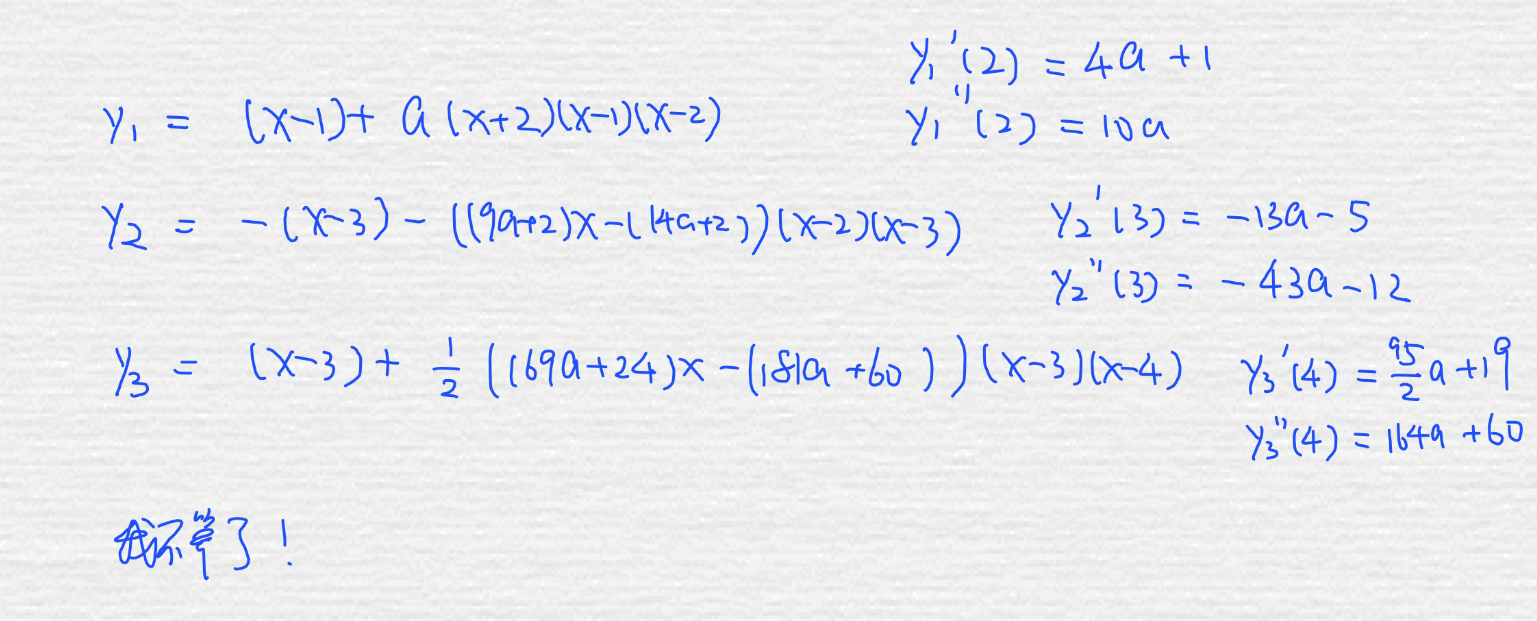
\includegraphics[scale=0.2]{figure.jpg}
        \caption{三次样条插值}
        \label{figure_spline}
    \end{figure}
    就算到这里吧.

    \subsubsection{Subfigrues}

    有换行的subfigure.

    \begin{figure}[H]
        \begin{subfigure}[b]{0.30\textwidth}
            \centering
            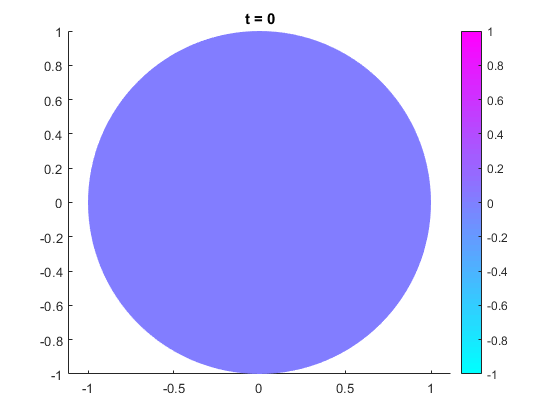
\includegraphics[width=\textwidth]{wc22.png}
            \caption{$u(x,y,0.0)$图像}
        \end{subfigure}
        \hfill
        \begin{subfigure}[b]{0.30\textwidth}
            \centering
            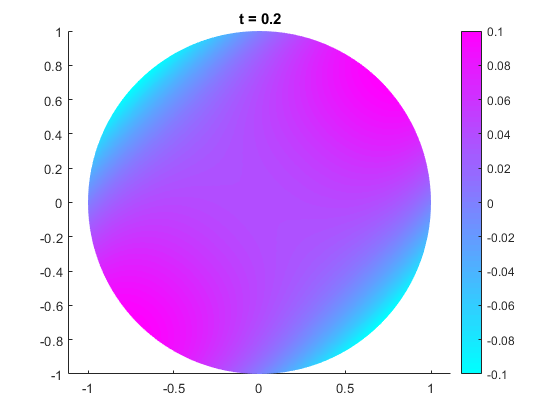
\includegraphics[width=\textwidth]{wc23.png}
            \caption{$u(x,y,0.2)$图像}
        \end{subfigure}
        \hfill
        \begin{subfigure}[b]{0.30\textwidth}
            \centering
            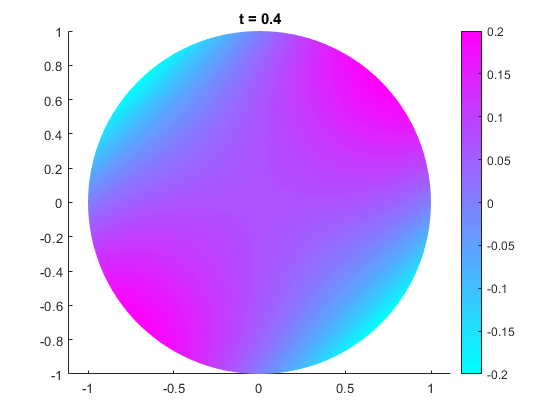
\includegraphics[width=\textwidth]{wc24.png}
            \caption{$u(x,y,0.4)$图像}
        \end{subfigure}
        
        \begin{subfigure}[b]{0.30\textwidth}
            \centering
            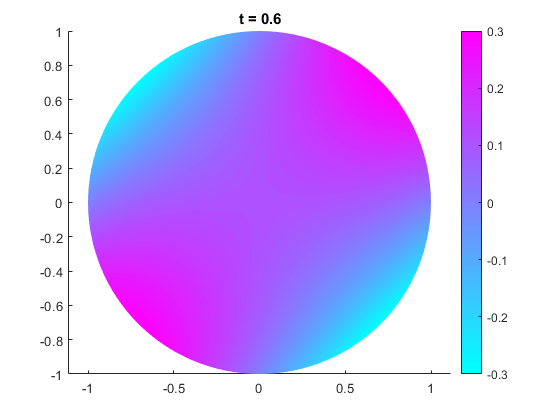
\includegraphics[width=\textwidth]{wc25.png}
            \caption{$u(x,y,0.6)$图像}
        \end{subfigure}
        \hfill
        \begin{subfigure}[b]{0.30\textwidth}
            \centering
            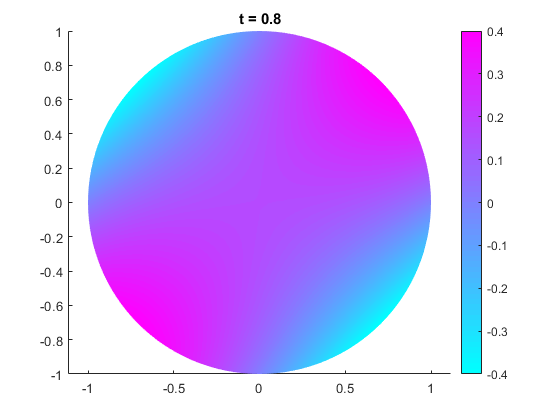
\includegraphics[width=\textwidth]{wc26.png}
            \caption{$u(x,y,0.8)$图像}
        \end{subfigure}
        \hfill
        \begin{subfigure}[b]{0.30\textwidth}
            \centering
            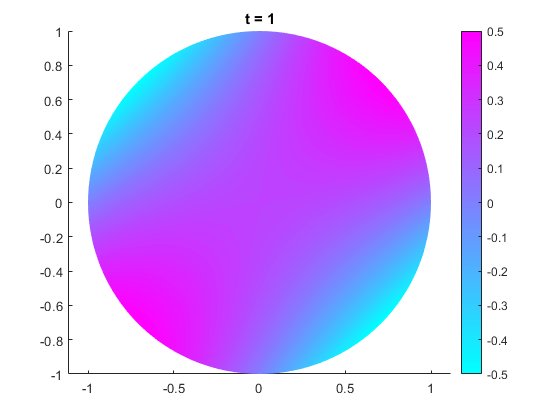
\includegraphics[width=\textwidth]{wc27.png}
            \caption{$u(x,y,1.0)$图像}
        \end{subfigure}
        \caption{问题2图像}
    \end{figure}

    \subsection{Tables}

    用笔算出\ref{table_13}中的自然三次样条插值.
    \begin{table}[H]
        \begin{center}
            \caption{习题中给定的三次样条数据}
            \label{table_13}
            \begin{tabular}{cccccc}
                \toprule
                $x$ & 1 & 2 & 3 & 4 & 5\\
                \midrule
                $y$ & 0 & 1 & 0 & 1 & 0\\
                \bottomrule
            \end{tabular}
        \end{center}
    \end{table}

    这次我们尝试用pgfplotstable包来画表格.
    \begin{table}[H]
        \begin{center}
            \caption{pgfplotstable}
            \pgfplotstabletypeset{
                a b
                5000 1.234e5
                6000 1.631e5
                7000 2.1013e5
                9000 1000000
            }
        \end{center}
    \end{table}

    \section{Mathematics}

    \subsection{Equations}

    \subsubsection{Aligned Equations with Brackets}

    \begin{equation}
        \left\{
        \begin{aligned}
            v'(t) &= g - \frac{c_{d}}{m}v^{2},\quad t\in [0, 10],\\
            v(0) &= 0,
        \end{aligned}
        \right.
    \end{equation}

    \subsection{Symbols}

    \subsubsection{Matrix and Vector}

    矩阵变量的写法以及转置的写法如下:
    \begin{equation}
        \matr{A}^{\top} =
        \begin{pmatrix}
            1 & 0\\
            0 & 1
        \end{pmatrix}
    \end{equation}

    向量$\vect{a}, \vect{b}^{\top}$即为所求.

    \subsubsection{Probability}

    The conditional expectation can be type-set like $\expect{X|Y}$.

    \subsection{Theorem}

    \begin{problem}
        记$\displaystyle a_n=\int_{0}^{1}{\frac{x^n}{\sqrt[3]{1-x}}\diff x}$,
        $\displaystyle b_n=\int_{\delta}^{1}{\frac{x^n}{\sqrt[3]{1-x}}\diff x}$.
        证明:
        \[\lim_{n\to \infty}{\frac{b_n}{a_n}}=
        \lim_{n\to \infty}{\frac{a_{n+1}}{a_n}}=
        \lim_{n\to \infty}{\sqrt[n]{a_n}}=1.\]
    \end{problem}

    \begin{solution}
        分别证明三个极限等于1.

        \begin{enumerate}[Step i.]
            \item

            证明$\sqrt[n]{a_n}\to 1$.\\
            根据Beta函数定义, 可知$a_n=\Beta(n+1, 2/3)$, 故有通项公式
            \begin{equation}
                a_n = \frac{3}{2}\prod_{j=1}^{n}{\frac{3j}{3j+2}}.
            \end{equation}

            首先有
            \begin{equation}
                \label{angeq}
                a_n
                \geq \frac{3}{2}\prod_{j=1}^{n}{\frac{3j}{3j+3}}
                = \frac{3}{2(n+1)}
            \end{equation}

            其次我们有
            \begin{equation}
            \begin{aligned}
                a_n &= \frac{\Gamma(n+1)\Gamma(2/3)}{\Gamma(n+5/3)}\\
                &= \frac{n!\cdot\Gamma(2/3)}{(2/3)\cdot(5/3)\cdot\dotsm
                    \cdot(n+2/3)\cdot\Gamma(2/3)}\\
                &\leq \frac{3}{2}\cdot n!.
            \end{aligned}
            \end{equation}
            故
            \begin{equation}
                1\leftarrow \sqrt[n]{3/(2(n+1))} \leq a_n
                    \leq \sqrt[n]{2/3\cdot n!} \to 1.
            \end{equation}

            \item

            证明$b_n/a_n\to 1.$\\
            记$\displaystyle f_n(x)=\frac{x^n}{\sqrt[3]{1-x}}$, $x\in [0, 1)$.
            因为$f_n>0$, 由单调收敛定理和黎曼瑕积分定义可知
            \begin{equation}
                (L)\int_{0}^{1}f_n = (R)\int_{0}^{1}f_n.
            \end{equation}

            故
            \begin{equation}
            \begin{aligned}
                a_n-b_n
                &=(L)\int_{0}^{\delta}{f_n(x)\diff x}\\
                &\leq (L)\int_{0}^{\delta}{f_n(\delta)\diff x}\\
                &= (R)\int_{0}^{\delta}{f_n(\delta)\diff x}\\
                &=\frac{\delta^{n+1}}{\sqrt[3]{1-\delta}}.
            \end{aligned}
            \end{equation}

            根据\ref{angeq}
            \begin{equation}
                \frac{a_n-b_n}{a_n}
                \leq\frac{\delta^{n+1}/(\sqrt[3]{1-\delta})}{3/(2(n+1))}
                \to 0
            \end{equation}

            即$b_n/a_n\to 1$.

            \item

            证明$a_{n+1}/a_n\to 1$.\\
            因为$a_n=\Beta(n+1, 2/3)$, 所以
            \begin{equation}
                \begin{aligned}
                    \frac{a_{n+1}}{a_n}
                    &= \frac{\Beta(n+2, 2/3)}{\Beta(n+1, 2/3)}\\
                    &= \frac{n+1}{n+1+2/3}\\
                    &\to 1.
                \end{aligned}
            \end{equation}
        \end{enumerate}
    \end{solution}

    \begin{proof}
        见\citep[P36]{rudin1976principles}.
        \citep[P34]{rudin1976principleschinese}
        \citep{rudin1976principleschinese2}
        \citep[ZBWDSB]{rudin1976principleschinese3}
    \end{proof}

    % -------------------- Bibliography --------------------

    \newpage
    \bibliography{bibliography}
    \bibliographystyle{plain}

\end{document}
